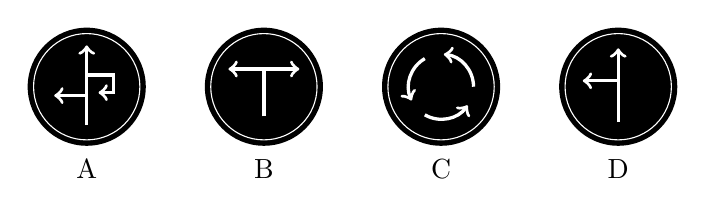
\begin{tikzpicture}[scale=.75]\foreach \x/\lab in {0/A,3/B,6/C,9/D}{\fill(\x,0)circle(1);\draw[white](\x,0)circle(.9);\node at(\x,-1.4){\lab};}\draw[white,very thick,->](0,-.65)--(0,.7);\draw[white,very thick,->](0,-.15)--(-.55,-.15);\draw[white,very thick,->](0,.2)--(.45,.2)--(.45,-.1)--(.2,-.1);\draw[white,very thick,->](3,-.5)--(3,.3)--(2.4,.3);\draw[white,very thick,->](3,.3)--(3.6,.3);\foreach \a in {0,120,240}{\draw[white,very thick,->](6,0)++(\a:.55)arc(\a:\a+85:.55);}\draw[white,very thick,->](9,-.6)--(9,.65);\draw[white,very thick,->](9,.1)--(8.4,.1);\end{tikzpicture}
